\section{程序设计与实现}

\begin{figure}[H]
  \centering
  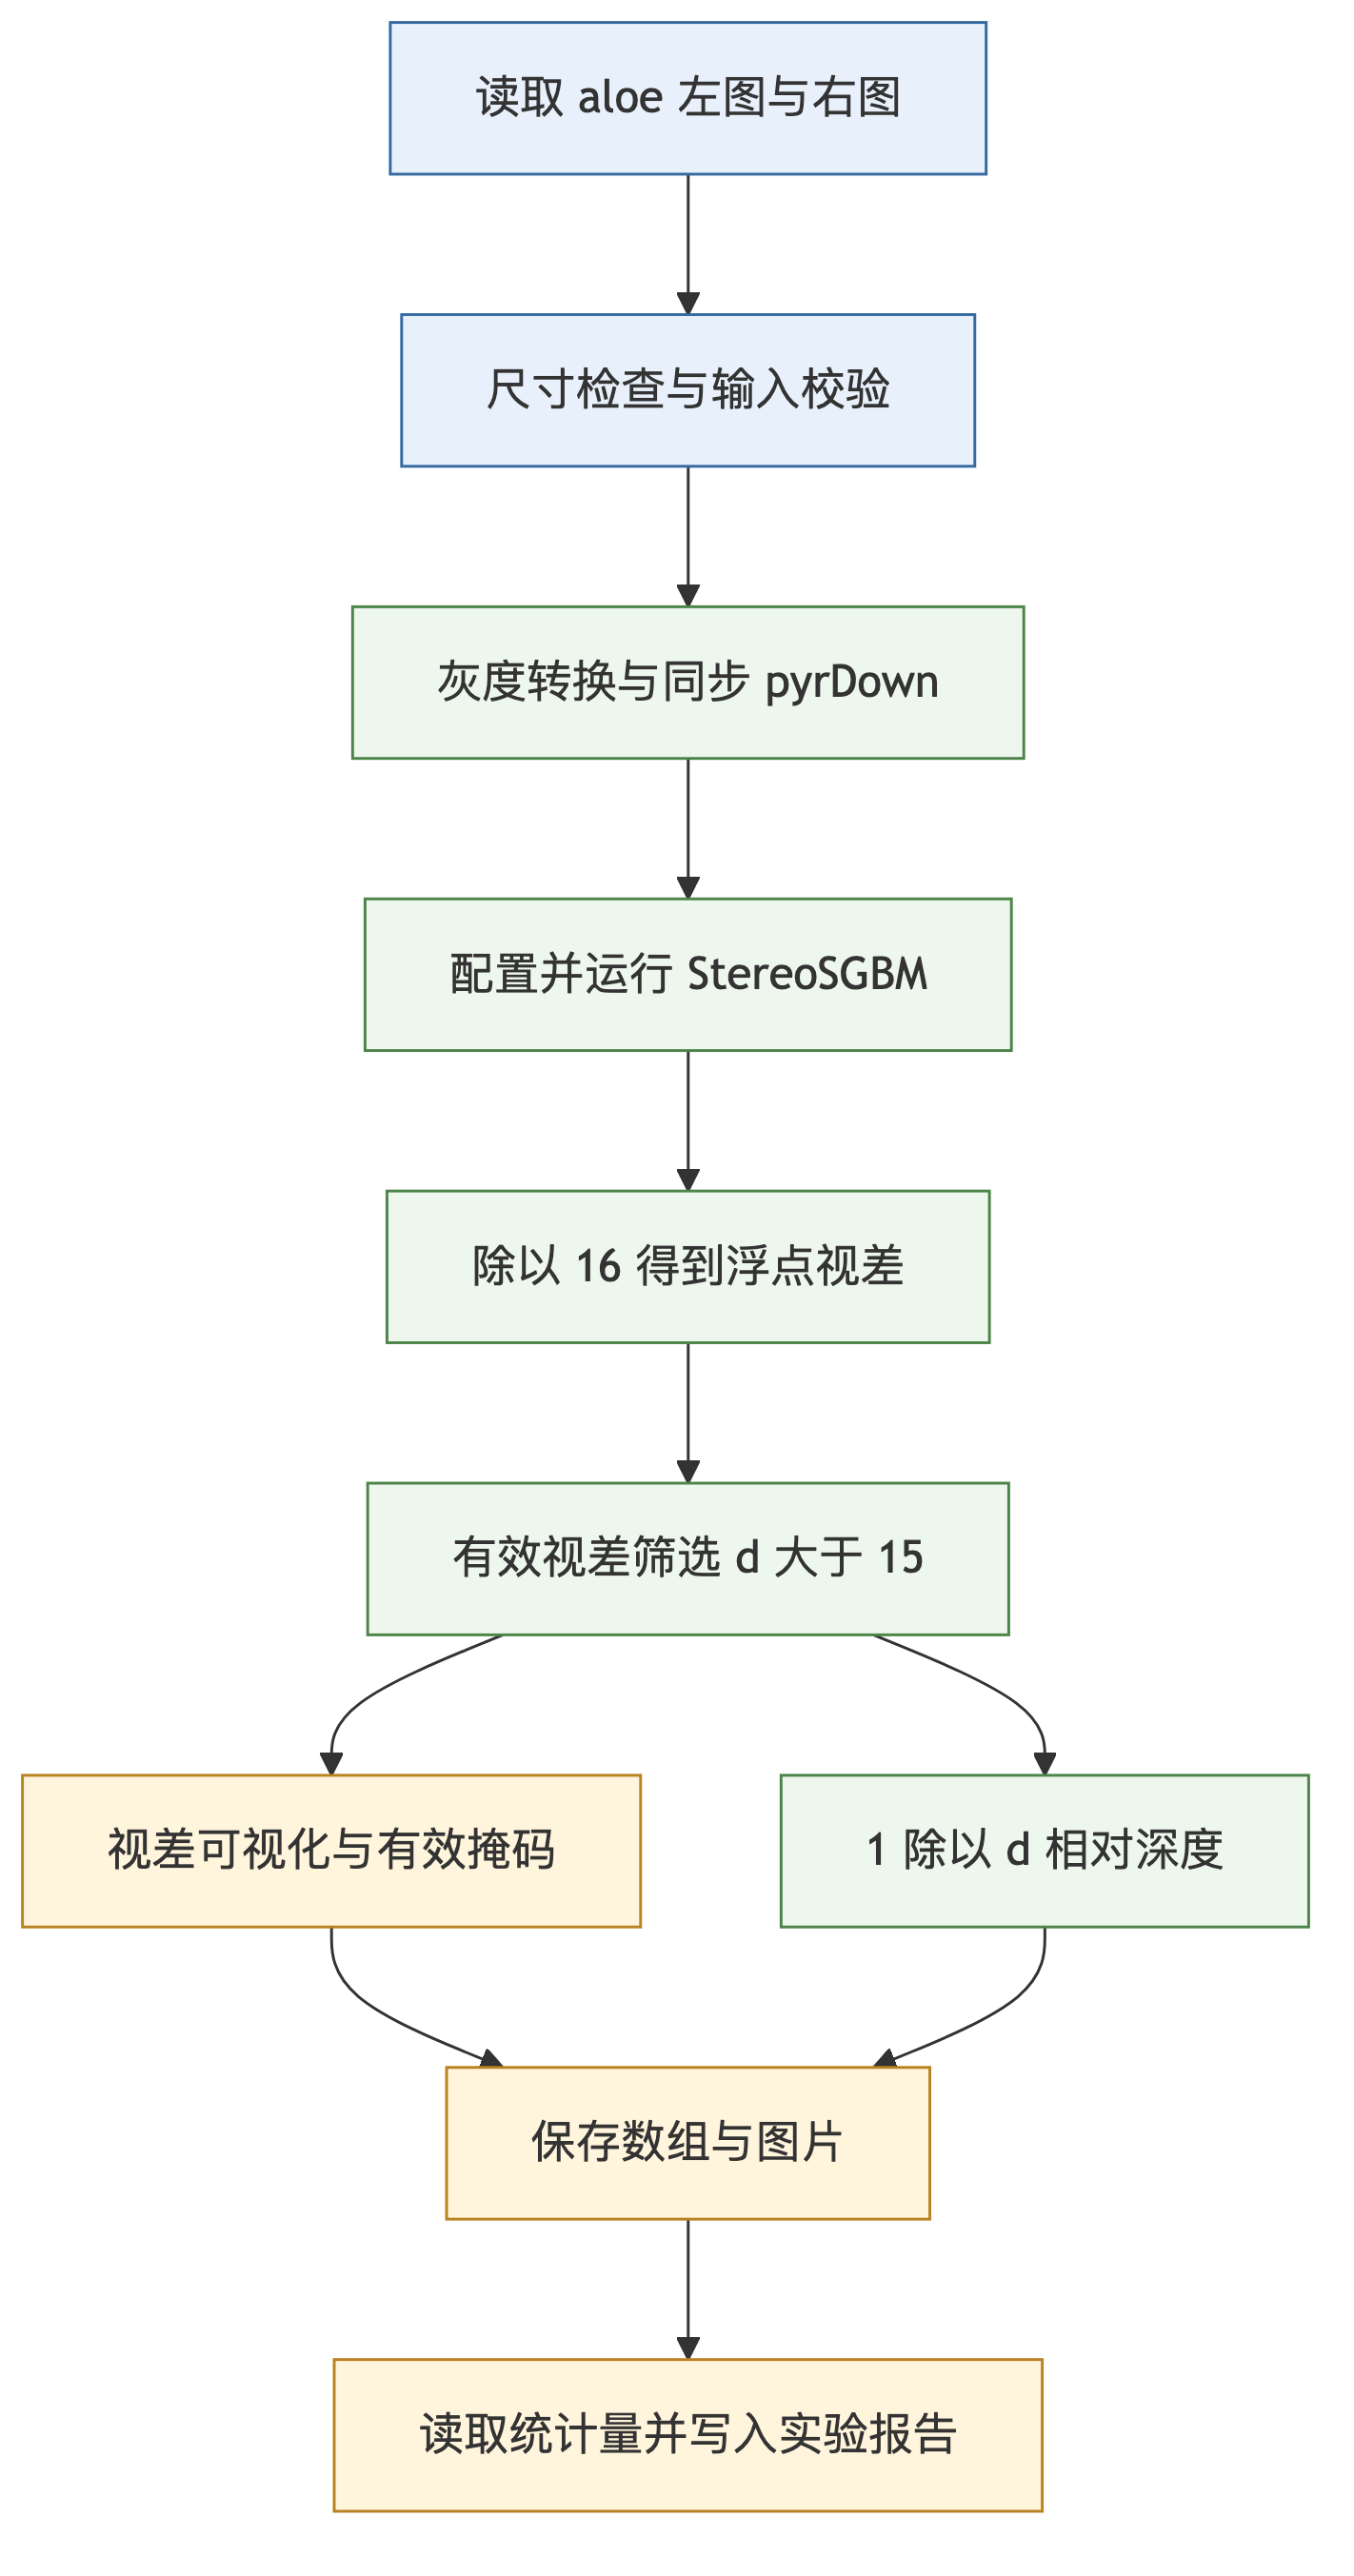
\includegraphics[height=0.72\textheight,keepaspectratio]{figures/stereo_pipeline.png}
  \caption{由 Mermaid 源文件生成的双目深度估计流程图。}
  \label{fig:stereo-pipeline}
\end{figure}

程序入口为 \codepath{task2/src/stereo_depth.py}，实现了从输入检查到结果落盘的单次
可复现实验。程序没有把显示图像当作数值输入，而是同时保存原始浮点数组和用于报告
的 8-bit 可视化。整体处理关系如图~\ref{fig:stereo-pipeline} 所示。

\subsection{输入读取、校验与预处理}

程序用 \texttt{cv2.imread} 读取左右彩色图像，并在匹配前检查：文件存在、OpenCV 返回非空
数组、左右图像的行列尺寸一致。尺寸不一致或图像为空时，程序直接抛出可定位的错误，
不会继续生成看似有效的结果。

随后将两幅图分别转换为灰度图。为降低计算量，左右彩色图和灰度图同步执行一次
\texttt{cv2.pyrDown}，因此不会引入左右不同的缩放比例。原始尺寸 $1282\times1110$ 变为
$641\times555$；所有后续视差数组和输出图片都对应这一处理尺寸。

\subsection{StereoSGBM 配置}

实际运行参数来自 \codepath{task2/results/params.json}，列于表~\ref{tab:sgbm-params}。
\texttt{numDisparities} 使用 16 的倍数，搜索范围覆盖官方 aloe 图像中主要的视差变化。

\begin{table}[H]
  \centering
  \caption{本次运行使用的 StereoSGBM 参数}
  \label{tab:sgbm-params}
  \begin{tabular}{lr}
    \toprule
    参数 & 实际值 \\
    \midrule
    \texttt{window\_size} & $3$ \\
    \texttt{minDisparity} & $16$ \\
    \texttt{numDisparities} & $96$ \\
    \texttt{blockSize} & $5$ \\
    $P_1$ & $72$ \\
    $P_2$ & $288$ \\
    \texttt{disp12MaxDiff} & $1$ \\
    \texttt{uniquenessRatio} & $10$ \\
    \texttt{speckleWindowSize} & $100$ \\
    \texttt{speckleRange} & $32$ \\
    \bottomrule
  \end{tabular}
\end{table}

\subsection{视差、有效掩码与相对深度}

OpenCV 匹配器返回带固定缩放的整数视差，程序除以 $16$ 得到像素单位的浮点数组。
本次有效条件为有限值且 $d>15$；不满足条件的位置在
\codepath{disparity_raw.npy} 中置为 \texttt{NaN}，从而不会参与范围、比例和相对深度统计。核心逻辑为：

\begin{lstlisting}[language=Python]
disparity = matcher.compute(left_match, right_match).astype(np.float32) / 16.0
valid = np.isfinite(disparity) & (disparity > 15)
disparity_raw = np.where(valid, disparity, np.nan)
depth_proxy = np.where(valid, 1.0 / disparity_raw, np.nan)
\end{lstlisting}

相对深度数组使用 $1/d$ 计算，单位为空，只用于表达相对前后关系。为了生成稳定的
显示图，程序只对有效像素取第 1 和第 99 百分位作为显示范围，再线性映射到 0--255；
因此 PNG 的灰度值不是原始视差或原始相对深度，定量分析必须回到 \texttt{npy} 数组。

\subsection{输出与异常检查}

程序在每次写文件后检查文件存在且非空。输出包括 \codepath{left.png}、\codepath{right.png}、
\codepath{disparity_raw.npy}、\codepath{disparity.png}、\codepath{valid_mask.png}、
\codepath{depth_proxy.npy}、\codepath{depth_proxy.png} 和 \codepath{params.json}。参数摘要还保存输入路径、处理尺寸、匹配器参数、
Python/OpenCV/NumPy 版本以及输出路径，保证报告数字可以回溯到同一批结果文件。
